\documentclass[11pt]{article} 
% CAMEL Grant: Phase I CAMEL-CN Proposal
% NSF 26-501: Collaboratory to Advance Mathematics Education and Learning for K-12
%
% The Proposal and Award Policies and Procedures Guide
% (PAPPG: https://www.nsf.gov/publications/pub_summ.jsp?ods_key=pappg)
% mandates, in Chapter 2, section B.2, that the main text should have a font size no less
% than 11 points for *most* typefaces (including Computer Modern Roman and Times (new) Roman).
%
\usepackage{bm} 
\usepackage{tabularx}
\usepackage{colortbl}
\usepackage{color} 
\usepackage[hidelinks]{hyperref}
\usepackage{graphicx} 
\usepackage{wrapfig} 
\usepackage{subcaption}
\usepackage{vmargin} 
\usepackage{mathrsfs}
\usepackage{float}
\usepackage{soul}
\usepackage{enumitem}
\linespread{0.901}
\usepackage[svgnames]{xcolor}  
\usepackage[most, breakable]{tcolorbox}   

\setlist[itemize]{noitemsep, topsep=8pt, parsep=0pt, partopsep=0pt}

% Define colors for highlighted boxes
\definecolor{mycmykcolor}{cmyk}{0, 0, 0.22, 0}
\definecolor{secondary}{cmyk}{0,0,0,0.20} 

\usepackage{titlesec}
\titleformat{\section}[runin]{\normalfont\bfseries}{\thesection}{1em}{}[]
\titlespacing*{\section}{0pt}{0.1\baselineskip}{1ex}

\titleformat{\subsection}[runin]{\normalfont\bfseries}{\thesubsection}{1em}{}[:]
\titlespacing*{\subsection}{0pt}{0.1\baselineskip}{1ex}

% Define a custom command to format section titles with a new line
\newcommand{\customsection}[1]{%
  \titleformat{name=\section,numberless}[runin]{\normalfont\bfseries}{}{0pt}{\newline}[ ]%
  \section{#1\newline}%
}


\usepackage{caption}
\usepackage{booktabs}
\usepackage[square,sort&compress]{natbib}
\bibliographystyle{unsrtnat}
\setcitestyle{numbers, square, comma, sort&compress}

%\hypersetup{colorlinks=true,linkcolor=blue,urlcolor=blue}

% Margins: at least 1 inch in all directions per PAPPG
\setpapersize{USletter}
\setmarginsrb{1in}{1in}{1in}{1in}{0pt}{0mm}{0pt}{0mm}

\pretolerance=5000
\tolerance=9000

\graphicspath{{/images/}} 

\newcommand{\pseudodot}{{\lower 2.4pt\hbox{$\cdot$}}}

\usepackage{lineno}

\begin{document}

\pagestyle{empty} % Commented out to show page numbers. Turn on at end

\setlength{\baselineskip}{12.6pt} 
\setlength{\normalbaselineskip}{12.6pt} 

%%%%%%%%%%%%%%%%%%%%%%%%%%%%%%%%%%%%%%%%%%%%%%%%%%%%%%%%%%%%%%%%%%%%%%%%%%%%%%%
% PROJECT DESCRIPTION BOX
%%%%%%%%%%%%%%%%%%%%%%%%%%%%%%%%%%%%%%%%%%%%%%%%%%%%%%%%%%%%%%%%%%%%%%%%%%%%%%%

\begin{tcolorbox}[colback=mycmykcolor, colframe=black, boxrule=1pt, coltext=black]

\textbf{Project Description:} 
This \textbf{Phase I} CAMEL Collaborative Network (CAMEL-CN) will address the lack of educational datasets documenting how K-12 learners navigate real-world datasets exhibiting statistical, structural, and provenance complexity, which are foundational capabilities for AI literacy.
This \textbf{Novel Dataset Pathway (1a)} project immerses high school students (Grades 9–12) in authentic data from AI infrastructure contexts, generating a multi-layered, AI-ready Student Math Modeling Learning Dataset.
These industrially relevant contexts introduce students to the entire ecosystem of AI deployment, from computing substrates to the cyber-physical energy systems that power them.
In doing so, we contribute to the national AI systems capacity as skilled, AI-literate Americans later enter the workforce.
By integrating researchers in learning sciences, education practitioners, and data scientists, this network bridges fundamental knowledge of human cognition and behavior with classroom practice to reveal new insights into how students develop mathematical modeling competencies through authentic complexity.
The resulting FAIR-compliant dataset will catalyze the development of AI-based formative assessment tools and intelligent tutoring systems while providing a replicable data translation framework for porting complex engineering research into K-12 curricula.

\end{tcolorbox}

%%%%%%%%%%%%%%%%%%%%%%%%%%%%%%%%%%%%%%%%%%%%%%%%%%%%%%%%%%%%%%%%%%%%%%%%%%%%%%%
% SECTION 1: INTRODUCTION
%%%%%%%%%%%%%%%%%%%%%%%%%%%%%%%%%%%%%%%%%%%%%%%%%%%%%%%%%%%%%%%%%%%%%%%%%%%%%%%

\section{Introduction:} 
Students leave school unable to work with real-world industrydata, and researchers lack the data to understand why because no educational dataset captures how students actually reason through authentic complexity.
The use of mathematics to represent, analyze, make predictions, or provide insight into real-world phenomena, which can be collectively described by the term ``mathematical modeling,'' is foundational to success in data science and AI-intensive careers.
Yet most students lack exposure to datasets that accurately represent authentic industrial and scientific contexts, which are ``messy.''
Instead, existing mathematics education datasets have been curated to control complexity in a way that reduces friction in teaching and learning.
This creates an important gap: students learn only to execute prescribed procedures and leave school unprepared to work with real-world datasets, while educational researchers lack the data necessary to understand how mathematical modeling competencies develop in these authentic contexts.

This Phase I CAMEL-CN will directly address this gap by integrating researchers from the science of learning, education practitioners, and data scientists to generate high-value datasets through the \textbf{Novel Dataset Pathway (Phase 1a)}.
We will pursue three interconnected sets of goals:
\textbf{Mathematics Learning Goals:} Students (Grades 9–12) will develop competencies in Algebra, Statistics, and mathematical modeling by making assumptions, identifying variables, creating, interpreting, and validating mathematical models, reasoning with uncertainty, and navigating trade-offs in real-world contexts.
\textbf{Math Education Research Goals:} Investigate student engagement and reasoning in authentic mathematical modeling problems situated in industrial AI contexts, identifying students' assets and obstacles when encountering authentic complex modeling.
\textbf{National AI Infrastructure Goals:} Generate a research-grade dataset to catalyze the development of AI-based formative assessment tools and intelligent tutoring systems.

%%%%%%%%%%%%%%%%%%%%%%%%%%%%%%%%%%%%%%%%%%%%%%%%%%%%%%%%%%%%%%%%%%%%%%%%%%%%%%%
% SECTION 2: BACKGROUND AND RATIONALE
%%%%%%%%%%%%%%%%%%%%%%%%%%%%%%%%%%%%%%%%%%%%%%%%%%%%%%%%%%%%%%%%%%%%%%%%%%%%%%%

\section{Background and Rationale:}

\subsection{Authentic Complexity in Mathematical Modeling}

The need for authentic, ``messy'' mathematical modeling experiences is well-established in education research~\cite{lesh2003foundations, Garfunkel2019}.
We use \textbf{messy} to describe students' phenomenological experience of interacting with data that is statistically complex, high-dimensional, and/or irregular due to provenance; the perceived difficulty that precedes analysis and insight.
This departs slightly from prior work~\cite{kjelvik2019getting} treating messiness as a property of a dataset: we argue that dataset-level features such as outliers, missingness, and variability are necessary components of, but distinct from, the phenomenological experience of mathematical reasoning with complex data.
Authenticity has been identified as a defining characteristic of mathematical modeling tasks~\cite{palm2007features, kaiser2017teaching}, with engagement in real-world data situations foregrounded as an important dimension of authenticity, particularly in data modeling activities. 

Despite this existing body of work, K–12 mathematics education predominantly relies on data sets that have been pre-cleaned and curated to reduce complexity.
While pedagogically useful for teaching isolated concepts, these data sets fail to prepare students for the authentic data challenges they will encounter in STEM careers and higher education.
Industrial and research data sets, such as those from materials processing, structural testing, and AI infrastructure, contain statistical complexity (sensor noise, measurement uncertainty), structural complexity (high dimensionality, correlated features), and provenance artifacts (missing values, data entry errors) that require qualitatively different reasoning strategies than those taught through textbook examples.~\cite{kjelvik2019getting}

In Pennsylvania, this gap is particularly acute. 
The Pennsylvania Core Standards for Mathematics \cite{pde2014pacoremath}, closely aligned with the Common Core State Standards, include the Model with Mathematics practice across all high school courses and call on students to interpret data, analyze linear models, and make inferences from statistical experiments. 
However, the content standards focus on clean, structured data, measures of center and spread, standard displays, line fitting, and correlation, with no explicit attention to data cleaning, provenance, measurement error, or multivariate reasoning. 
The modeling cycle examples embedded in the standards (stopping distance, savings account balance, bacterial growth) are largely deterministic or idealized, and the content standards do not scaffold students into working with authentic data from STEM contexts. 
At a national level, GAISE II \cite{Bargagliotti2020}, which is endorsed by the National Council of Teachers of Mathematics, and GAIMME \cite{Garfunkel2019} call for high school students to engage in more authentic mathematical modeling.
A 2023 National Academies workshop proceedings~\cite{NASEM2023} and a 2025 IES white paper~\cite{IES2025} both called for research into student experiences in data management and analysis. 

% seems unnecessary
% The CAMEL initiative explicitly calls for datasets that are ``representative of all K-12 learners,'' ``AI-ready,'' and capable of advancing research on math learning.
% This project addresses the current deficiency: the absence of large-scale data documenting how students transition from abstract mathematics to the ``messy'' reality of industrial engineering and data science.

\subsection{Science of Learning Foundations}

% Mathematical modeling competencies develop differently when students encounter authentic constraints -- statistical complexity arising from measurement variance, structural complexity arising from dimensionality, and provenance artifacts reflecting practical realities of data collection -- versus sanitized textbook examples because authentic modeling shifts the work from executing predetermined procedures to making and justifying decisions throughout the modeling cycle.
In mathematics modeling literature, empirical syntheses emphasize that students’ growth in modeling competencies is tightly linked to opportunities to formulate assumptions, identify variables, create and coordinate representations, interpret results in context, and validate or refine models when the data do not ``behave'' ideally~\cite{schukajlow2018empirical, cevikbas2022systematic}.
When datasets are messy, these competencies become more visible and more necessary since students must decide how to treat statistical complexity and compare alternative modeling pathways (e.g., different functional forms, summaries, or feature sets) while defending why a particular approach is warranted. 
Studies show that students working with authentic datasets exhibit sophisticated reasoning about variability, constraint-setting, and trade-offs that is largely absent with pre-cleaned data, bolstering the idea that data preparation is an essential step within modeling~\cite{wilkerson2022exploring, english2018modelling}.
% In data modeling activities, learners' navigation of ambiguity is visible in how they set constraints, select variables, justify trade-offs, and defend non-unique solutions in particular when tasks use real performance data or other messy sources rather than sanitized textbook numbers~\cite{english2018modelling}. 
% Related work on novices’ engagement with big data highlights how uncertainty is not merely a context feature but a reasoning object.
When working with big data, students need to articulate sources of uncertainty and reconcile competing signals, which naturally drives them toward iterative interpretation~\cite{gafny2025novices}. 
% Authentic, data-rich modeling is also diagnostically powerful because it surfaces persistent misconceptions that can remain hidden in idealized exercises. 
Research also documents robust misconceptions about sampling and inference, such as treating samples as deterministic ``miniatures'' without accounting for sampling variability, or misinterpreting what inferential claims can and cannot warrant~\cite{saldanha2002conceptions, sotos2007students}.
In algebra, students' misconceptions are common and persistent~\cite{knuth2005middle}, and become consequential when students must make decisions and interpret results in the context of real systems. 

\subsection{A Framework for Data Complexity}
This proposal addresses three interconnected notions of complexity: that of statistical, structural, and provenance.
Statistical complexity (mostly properties of the distributions) can appear in textbook settings, but is often reverse-engineered for that use case.~\cite{kerlin2010complexity, kjelvik2019getting}
Structural complexity (high dimensionality, irrelevant variables) and provenance artifacts (irregularities and missing values arising from human-in-the-loop data collection) are more rarely used due to the problems they pose in statistical analysis.~\cite{berland2010learning, gould2014praise}
Surveys indicate that messy data curation is entirely omitted by most instructors.~\cite{legacy2022computes, konold2000engaging}
Provenance is especially important in the context of authenticity, as the complexity arises precisely because the data originated in the real world and passed through real laboratory or industrial protocols.
These aspects will be absent from sanitized datasets by both intent and definition~\cite{hardin2018dynamic}.
This stands at odds with the up to 80\% of professional data scientists' efforts being tied up in so-called ``janitorial'' data work~\cite{donoho201750, lohr2014big}. 

\subsection{The Case for Process-Level Learning Data}

The most comprehensive existing datasets each capture product data from structured problem-bank or closed-interface environments, with no student-generated code, limited exposure to authentic datasets, and no process-level trajectories. In essence, they reveal whether a student arrived at the right answer, but not how they got there. In brief: ASSISTments \cite{feng2009addressing} is the largest publicly available K-12 math dataset with approximately 500,000 students and over 10 million problem attempts, capturing clickstream data from an intelligent tutoring system; PSLC DataShop \cite{koedinger2010data} provides comprehensive learning analytics from Carnegie Learning's Cognitive Tutor systems; TIMSS \cite{mullis2012timss} and NAEP \cite{nces2012naep, nces2012naep_science} provide only final answers and limited constructed responses. Each of these treats the student's reasoning process as a black box: they reveal whether a student arrived at the right answer, but not how they navigated the ambiguity that authentic modeling requires.

\begin{wrapfigure}{r}{0.6\linewidth}
    \vspace{-4mm}
    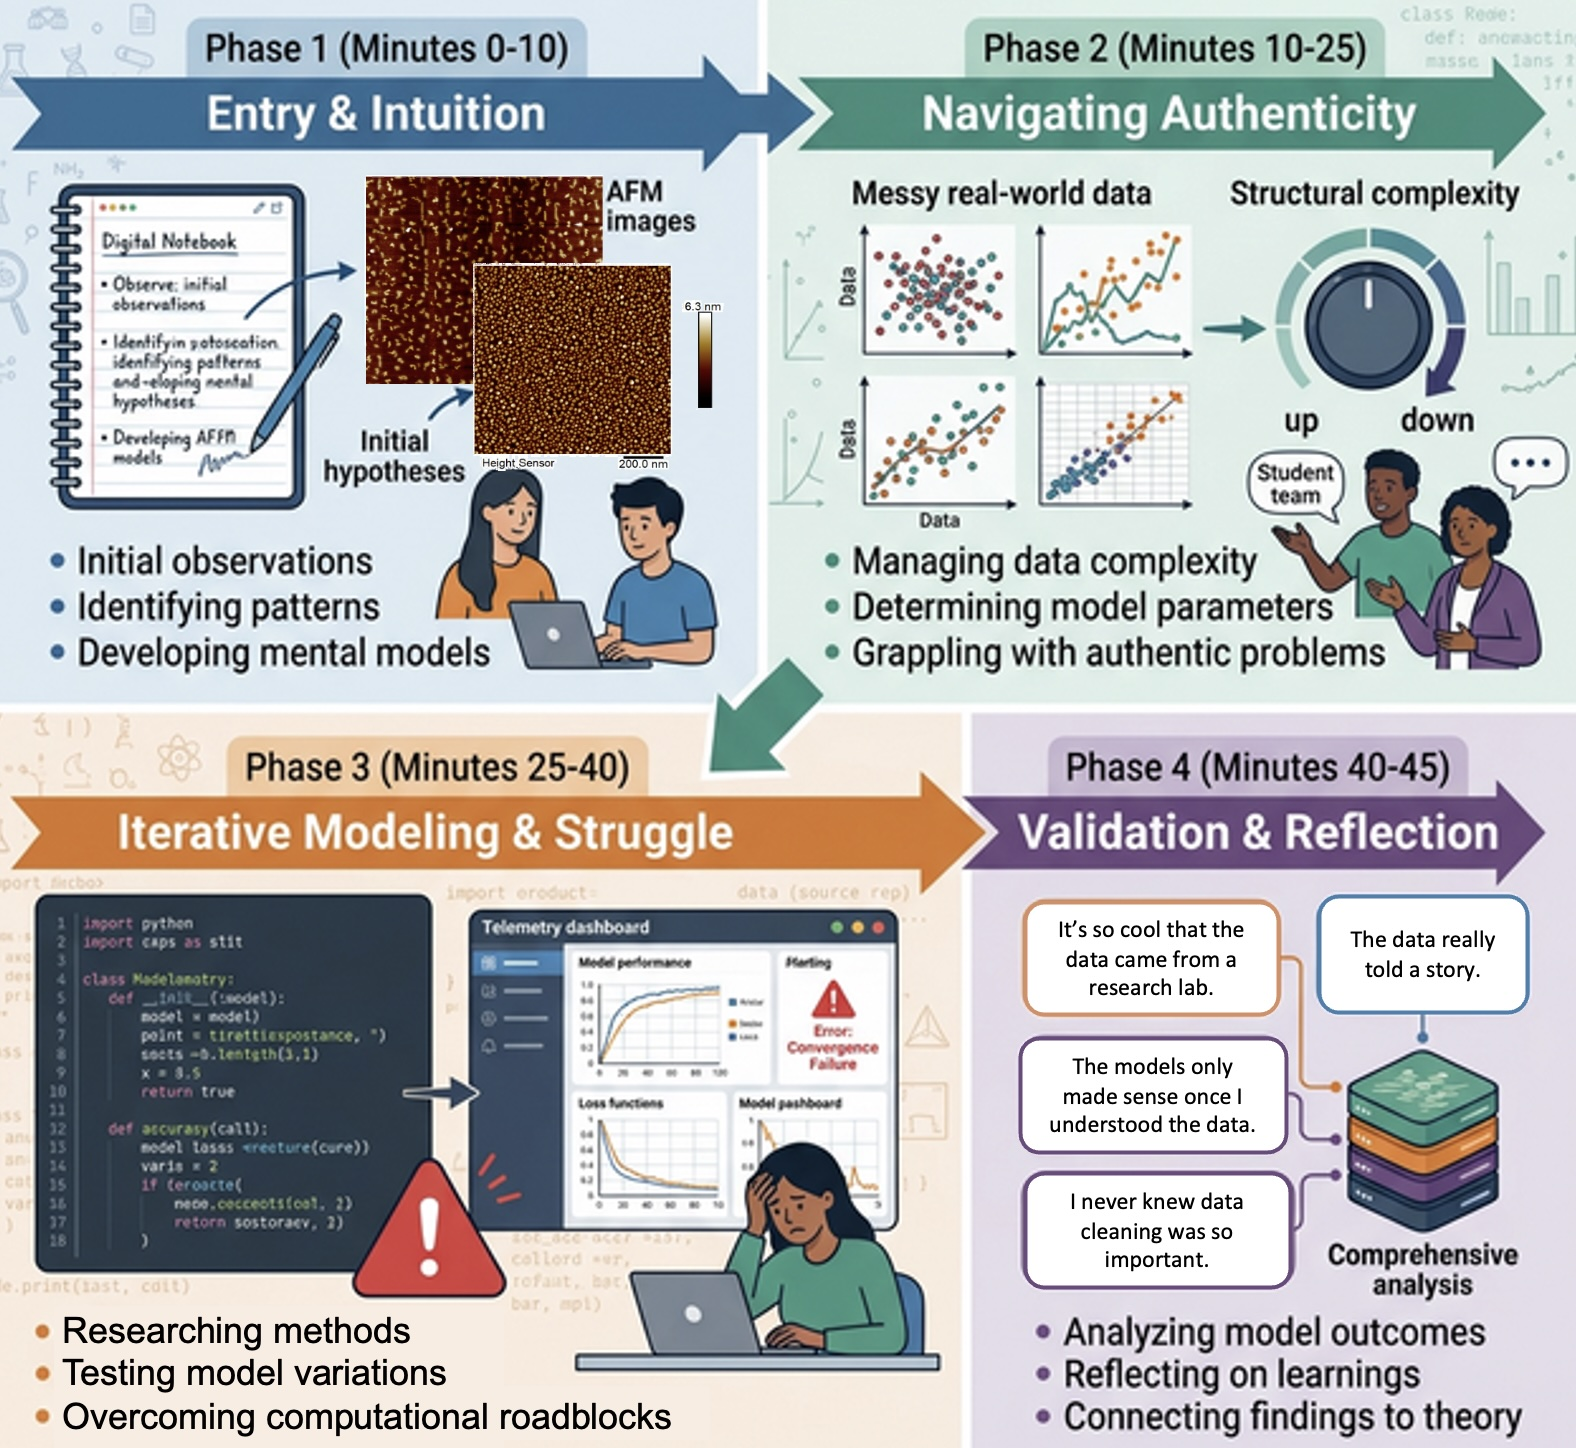
\includegraphics[width=\linewidth]{images/student_experience_v2.jpg}
    \caption{Schematic representation of the student experience during a 45-minute modeling cycle. Live telemetry from Jupyter notebooks will capture longitudinal process data as students reason.}
    \label{fig:experience}
    \vspace{-2mm}
\end{wrapfigure}

The literature establishes why this black box is consequential: complex data contexts can support conceptual understanding precisely because they force students to connect mathematical structure with contextual meaning. In these settings, variability becomes something to be interpreted rather than dismissed, parameters require contextual explanation, and models are evaluated through evidence rather than predetermined answers. These moments can be intentionally leveraged as opportunities for productive struggle, thereby supporting deeper conceptual learning and more adaptive expertise than approaches that prioritize immediate procedural success \cite{kapur2012designing, kapur2016examining}. What the literature is working to establish, because the data do not exist, is how productive struggle unfolds behaviorally in open-ended computational modeling tasks. Process-level capture is the prerequisite capability to enable researchers to reconstruct the trajectory rather than just the destination \cite{winne1998studying, baker2014educational}.

While traditional laboratory-based research leverages multimodal learning analytics (MMLA) to provide objective reconstruction of the learner's journey through hardware such as eye-tracking \cite{hao2025process, zhao2021role} and physiological sensors \cite{possaghi2025integrating, leecultura2023multimodal}, these are difficult to scale to thousands of students in diverse settings. 
This project addresses this limitation by translating the goals of MMLA into a scalable, digital framework.
Instead of physical sensors, this methodology leverages high-resolution data streams, including trace logs that document step-by-step digital interactions \cite{acosta2024multimodal} and code execution patterns.
Within computational modeling contexts, Monte Carlo Tree Search (MCTS) combined with code-augmented verification enables the generation of step-by-step reasoning trajectories, allowing researchers to validate the logical consistency of a student's struggle through executable code rather than chance \cite{guan2025rstar, lin2025scaling}. 
By tracking digital pathways, such as the transition from confusion to ``serious engagement with impasse," this capability identifies behavioral markers of productive struggle that are typically obscured in traditional assessment frameworks \cite{riegel2021frustration, goldin2000affective, possaghi2025integrating}.

% \hl{PLACEHOLDER - BECCA/WES: Add 2-3 citations on learning analytics, process-level data capture, and Python-based education research}

%%%%%%%%%%%%%%%%%%%%%%%%%%%%%%%%%%%%%%%%%%%%%%%%%%%%%%%%%%%%%%%%%%%%%%%%%%%%%%%
% SECTION: PRIOR NSF SUPPORT
%%%%%%%%%%%%%%%%%%%%%%%%%%%%%%%%%%%%%%%%%%%%%%%%%%%%%%%%%%%%%%%%%%%%%%%%%%%%%%%

\section{Results from Prior NSF Support:}

\textbf{Rebecca Napolitano}, \textbf{Kathy Hill}, and \textbf{Wesley Reinhart} share prior support from ``Collaborative Research: HDR DSC: Infusion of data science and computation into engineering curricula'' (PI and Co-PI, respectively, IIS-2123343, \$1,127,957, 10/21–9/26).
\textit{Intellectual Merit:} A curricular framework for data science education created with community stakeholders and industry partners. 
\textit{Broader Impacts:} An evidence-based blueprint for best practices in integrating data science with engineering curricula. 
\textit{Research Products:} This ongoing work has resulted in academic dissemination, including educational research \cite{asdetranslating2023, solnosky2024wip, reinhart2025opinion, napolitano2025analyzing} and domain-specific research used to collect data for the curriculum \cite{farnod2022damage, farnod2023displacement, farnod2025damage, upadhyay2025data, kumar2025bio, oturak2026data, paulino2021grammar, paulino2022reviver, paulino2023automating, saleem2023analysis,     whitesides2023research, kaushal2026historic,napolitano2026shm, duan2026preserving, napolitano2025preserving, maalouf2025assessment, paulino2025data, blain2025nheri, kallas2025understanding, kallas2025beyond, napolitano2025analyzing, maalouf2025community, kallas2025image, napolitano2025educational, reinhart2025opinion, farnod2025damage, saleem2025comparative, alam2024data, paulino2024determining, kaushal2024three, chen2024addressing, kaushal2024assessing, kallas2024understanding, saleem2024evaluating, kaushal2023understanding, laflamme2023roadmap, kallas2023image, kallas2023automated}
Additionally, this ongoing work has resulted in a website that provides information about a data science program offering six courses tailored for engineering students.
% This project developed and validated a curricular framework for integrating community-centered data science and computation into undergraduate engineering programs.
% The team implemented and refined instructional approaches across multiple engineering disciplines, generating empirical evidence regarding how real-world datasets, with their inherent statistical, structural, and provenance complexity, can be structured to support learning while maintaining authenticity. 
% Key products include peer-reviewed publications on translating engineering data into educational contexts and the development of six complete data science courses for engineering students, which are now publicly available with accompanying Jupyter notebook modules.
The team prepared domain-specific datasets from building systems and materials science for classroom use, creating a small-scale precedent for the larger dataset generation effort proposed here.
% Four key insights from this prior work directly shape the current proposal. 
% First, data translation is non-trivial; converting research data for educational use requires systematic protocols and explicit decision-making about which complexities to preserve versus simplify, as ad-hoc cleaning produces materials that are either too sanitized to be authentic or too overwhelming to be accessible. 
% Second, we discovered that process data is essential, as student outcome measures alone do not capture how students engage with data complexity, leaving researchers unable to distinguish productive struggle from unproductive confusion. 
% Third, practitioner partnership is important, as curricula developed primarily by researchers without deep practitioner input on implementation realities face significant friction during classroom deployment. 
% Finally, we concluded that high school is the optimal context for this intervention because undergraduate students often arrive with entrenched expectations that ``real" data should be clean; intervening at the K-12 level offers greater potential to shape foundational data reasoning before these expectations calcify.
Four insights from this work directly shape the current proposal:
data translation requires systematic protocols (ad-hoc cleaning produces materials that are either too sanitized or too overwhelming);
student outcome measures alone cannot distinguish productive struggle from unproductive confusion, making process-level capture essential;
practitioner input is necessary to avoid significant friction during classroom deployment;
and undergraduate students often arrive with entrenched expectations about data, making K-12 intervention especially effective.

\textbf{Wangda Zuo} has prior support from ``Big Data Analytics for Optimized Planning of Smart, Sustainable, and Connected Communities'' (PI, IIS-1633338 and IIS-1802017, \$443,867, 2016-2022). \textit{Intellectual Merit:} to create an integrated modeling platform to study the interaction of energy, transportation, and communication \cite{tian2017coupling,he2016virtual, tian2017coupled, tian2018building, tian2018optimization, ye2018creation, zhou2018modelling, he2016towards, sevilla2018low, zhang2020predictive, lu2019open, anbarasu2024exploring}. 
\textit{Broader Impact:} to create a big data platform and open source virtual testbed based on a real-world net zero energy community in Florida to engage the broader community across various smart cities.
\textbf{Xiangquan Yao} has no prior NSF support.

%%%%%%%%%%%%%%%%%%%%%%%%%%%%%%%%%%%%%%%%%%%%%%%%%%%%%%%%%%%%%%%%%%%%%%%%%%%%%%%
% SECTION 3: NETWORK COMPOSITION
%%%%%%%%%%%%%%%%%%%%%%%%%%%%%%%%%%%%%%%%%%%%%%%%%%%%%%%%%%%%%%%%%%%%%%%%%%%%%%%

\section{Network Composition:}

This project's network integrates the three essential disciplinary perspectives required for CAMEL: researchers in the science of learning, education practitioners, and disciplinary data scientists.
The network is designed to enable new insights into mathematical modeling development that could not emerge from any single disciplinary perspective.
To ensure the successful execution and evaluation of this Phase I network, the team will adhere to a structured Collaboration and Management Plan (see supplementary document).

% \begin{table}[h]
% \footnotesize
%     \centering
%     \vspace{-0.25cm}
%     \caption{Network composition and roles; specific PA schools listed in \autoref{tab:school_recruitment_data}}
%     \vspace{-0.25cm}
%     \begin{tabular}{|p{4cm}|p{4cm}|p{6.5cm}|}
%     \hline
%     \rowcolor{mycmykcolor}
%          \textbf{Team Member}  & \textbf{Expertise} & \textbf{Role in Network} \\
%          \hline
%          Rebecca Napolitano (Lead) & Computational Methods, Python-based Data Science Education & Lead Data Scientist; Data Translation; AI-ready annotation protocols \\
%          \hline
%          Xiangquan Yao (James) & Cognitive Science, Learning Sciences & Science of Learning Lead; Data collection protocol design \\
%          \hline
%          Wesley Reinhart & Materials Science, ML, Materials Informatics & Data Originator (Materials Processing); FAIR compliance \\
%          \hline
%          Wangda Zuo & Cyber-physical Systems, Energy Modeling & Data Originator (AI Infrastructure); Industrial dataset curation \\
%          \hline
%          CSATS Team and Partner Schools & Science Education, K-12 Partnerships & Practitioner Implementation; Standards alignment \\
%          \hline
%          Robert Mayne & K-12 Math Education, Policy & Practitioner Lead; Curriculum development; Teacher PD \\
%          \hline
         
%     \end{tabular}
%     \label{tab:team}
%     \vspace{-0.25cm}
% \end{table}

\textit{\textbf{Engineering and Data Science Research Partners:}} 
Wesley Reinhart (Materials Science \& Engineering, Penn State) and Wangda Zuo (Architectural Engineering, Penn State) serve as the primary data originators.
Their research programs are rooted in AI-guided discovery and provide a unique perspective on messiness in the context of real-world data artifacts.
By leveraging their expertise in scientific machine learning and large-scale data architecture, the project ensures that the instructional datasets are authentic and structured for the analytical demands of learning science research.
Reinhart will leverage large, authentic datasets from the 2D Crystal Consortium Materials Innovation Platform (2DCC-MIP) that has been operating for a decade.
2DCC-MIP is an NSF-funded national user facility focused on the development of highly specialized two-dimensional chalcogenide materials for next-generation electronics.
These datasets are already being packaged for data science training in service of the facility's educational mission, and can be readily adapted to new education contexts via Reinhart's ``Composable Courseware'' (CC) architecture, drawn schematically in \autoref{fig:composable-courseware}.
Reinhart also has experience adapting research datasets for data science training as Co-PI of an NSF National Research Traineeship at Penn State involving materials informatics.
Zuo will provide high-dimensional time-series datasets from NSF-funded cyber-physical research, including a campus-scale district cooling network and a university data center cooling system. 
These datasets introduce students to messiness through sparse metering in aging infrastructure, physically inconsistent readings under low-flow conditions, and high-frequency anomalies caused by abrupt, control-driven mode changes. 
By navigating these energy-materials nexus datasets, students must reconcile competing signals and operator-driven decisions that are often embedded within the raw data rather than defined by prescribed algorithms.

\textit{\textbf{Lead Data Scientist and Translation Lead:}}
Rebecca Napolitano (Architectural Engineering, Penn State) will serve as the network's Lead Data Scientist and Translation Lead.
Bringing expertise in computational methods and Python-based data science education, Napolitano will manage the conversion of complex engineering data streams into educator-ready Python frameworks while designing AI-ready annotation protocols.

\textit{\textbf{Science of Learning and Research Lead:}}
Xiangquan (James) Yao will direct the research program, applying cognitive science theories to the design of data collection protocols.
He will ensure that the protocols capture fine-grained student reasoning and engagement data in authentic modeling problems, meeting the highest standards for both educational research and machine learning communities.
He will employ multimodal learning analytics that integrate process-level interaction logs, intermediate modeling artifacts, and structured reflection prompts.

\textit{\textbf{Education Practitioners and Implementation Team:}}
Kathleen Hill, Director of the Center for Science and the Schools (CSATS), serves as the Practitioner Implementation Lead, managing K-12 partnerships and administrative relationships with rural districts. Robert Mayne, Einstein Distinguished Educator Fellow and Practitioner Development Adviser, leads the design of teacher professional development (PD) modules and oversees curriculum standards alignment. Together, Hill and Mayne ensure implementation fidelity and pedagogical quality.
Amber Cesare, CSATS Curriculum Integration Specialist, provides expertise in mathematical and scientific modeling. She serves as the primary field liaison, tuning the curriculum’s “complexity dials” to ensure that engineering datasets are appropriately scaffolded for high school learners without sacrificing authentic reasoning. A CSATS Computational Education Specialist (to be hired) will provide field-level quality control, ensuring that telemetry hooks and student-led data logging function correctly during classroom implementation.
Supporting the network’s coordination, Jeff Remington (CSATS Outreach Liaison) serves as the point of contact for school administrators. He facilitates the Networked Evaluation and Improvement Community (NEIC), a monthly forum where participating Rural Math Teachers (acting as Co-Researchers) collaborate with the research team to evaluate student performance evidence through iterative Plan-Do-Study-Act (PDSA) cycles.
%%%%%%%%%%%%%%%%%%%%%%%%%%%%%%%%%%%%%%%%%%%%%%%%%%%%%%%%%%%%%%%%%%%%%%%%%%%%%%%
% RESEARCH QUESTIONS BOX
%%%%%%%%%%%%%%%%%%%%%%%%%%%%%%%%%%%%%%%%%%%%%%%%%%%%%%%%%%%%%%%%%%%%%%%%%%%%%%%

% Research Questions
\section{Intellectual Merit:}

The intellectual merit of this work is twofold: advancing understanding of precisely how students develop mathematical modeling competencies with real-world data, while simultaneously establishing the methodological infrastructure that enables such research at scale.
The newly formed network will enable the investigation of questions that require convergence of learning sciences, data science, and practitioner perspectives.

\subsection{Research Questions}
The intellectual merit arises via two research questions that have been unanswerable until now because the process-level data required to study how modeling competencies develop in authentic industrial contexts do not exist. Existing datasets record only outcomes; this project is designed from the ground up to capture the reasoning in between:
\vspace{-0.2cm}
\begin{tcolorbox}[colback=mycmykcolor, colframe=black, boxrule=1pt, coltext=black]
\textbf{RQ1:} How do students develop mathematical modeling competencies when engaging with complex industrial datasets in Algebra and Statistics contexts?
\end{tcolorbox}
\vspace{-0.1cm}
% This question probes the core learning phenomenon at the heart of CAMEL's mission: understanding how K-12 students reason about authentic complexity. 
We will examine how students formulate problems, select and represent variables, construct and refine models, and validate model adequacy when working with authentic, complex datasets characterized by complexities inherent in real-world industrial contexts.
We will also examine the reasoning patterns, iterative strategies, and validation approaches that support productive engagement across modeling phases rather than isolated solution steps.
By documenting the assets students bring to these tasks, such as prior knowledge, intuitions about physical systems, computational problem-solving strategies, and the challenges they encounter, including misconceptions about uncertainty, difficulties navigating high-dimensional feature spaces, we will trace how mathematical modeling competencies develop through repeated cycles of model construction, evaluation, and revision in contexts that mirror real-world STEM practice.
% This work also examine how Python-based data science literacy emerges as an integral component of the modeling process, supporting data exploration, model testing, and evidence-based justification,and how sustained engagement with industrial data contexts shapes students' understanding of AI and data-driven STEM practices and career pathways.
% The question addresses a fundamental gap: existing research on mathematical modeling predominantly studies student work with sanitized textbook problems, leaving unexplored how competencies transfer to the realities of STEM careers.

\begin{tcolorbox}[colback=mycmykcolor, colframe=black, boxrule=1pt, coltext=black]
\textbf{RQ2:} What infrastructure, such as data translation frameworks and AI-ready annotation protocols, is required for the large-scale study of mathematical modeling with authentic data?
\end{tcolorbox}

% This question positions methodological infrastructure as a legitimate research contribution in its own right.
% The Data Translation framework will address a documented challenge from our prior NSF work: converting complex engineering research data into pedagogically accessible materials requires systematic protocols, rather than ad-hoc cleaning.
% We investigate which features of such a framework preserve essential complexity (realistic measurement error, ambiguous modeling choices) while ensuring high school accessibility through ``complexity dials'' that allow teachers to adjust difficulty without eliminating authenticity.

The Data Translation Framework is conceptualized as a theoretical model for the systematic preservation of authentic complexity across educational contexts.
We hypothesize that by utilizing a structured rubric of ``complexity dials," manipulating statistical, structural, and provenance complexity, researchers can identify the specific threshold where data-driven friction transitions from productive struggle into cognitive overload.
By evaluating this hypothesis, the field will gain generalizable evidence for how to scaffold ``messy'' real-world datasets in high school education.

Equally important is understanding what annotation and metadata structures make process-level learning data usable for training intelligent tutoring systems and formative assessment tools.
This requires integrating perspectives from learning scientists (what reasoning patterns matter?), data scientists (what representations enable machine learning?), and practitioners (what codes are interpretable for teachers?).
The interdisciplinary collaboration itself becomes a focus of study: how do disciplinary perspectives shape what we see in student data, and how does co-design of infrastructure strengthen both the dataset and the research insights it enables?

% Together, these questions address CAMEL's dual mandate: RQ1 advances learning science by revealing how mathematical modeling develops in authentic contexts, while RQ2 establishes methodological resources that enable the broader research community to conduct similar investigations.
% The network's convergent expertise is essential to both: understanding student learning with industrial data requires cognitive scientists who understand reasoning development, data scientists who recognize authentic complexity, and practitioners who can implement with fidelity.
% Similarly, building reusable infrastructure requires this same convergence to ensure frameworks are theoretically grounded, technically sound, and pedagogically viable.

\subsection{Theoretical Mechanism of Productive Struggle} 
The CAMEL-CN framework operates on the hypothesis that sanitized data reduces the friction of learning to the point of eliminating the very reasoning moves required for STEM careers.
Through authentic messiness, we trigger specific cognitive processes that idealized datasets cannot support:
\begin{table}[H]
    \centering
    \footnotesize 
    \caption{Theory of Change: Mapping Statistical, Structural, and Provenance Complexity to Student Outcomes and Behavioral Telemetry Signals}
    \vspace{-0.2cm}
    \label{tab:complexity_toc} 
    \renewcommand{\arraystretch}{1.4} 
    
    \begin{tabularx}{\textwidth}{|X|X|X|X|X|}
        \hline
        \rowcolor{mycmykcolor}
        \textbf{Inputs} & \textbf{Activities} & \textbf{Outputs} & \textbf{Outcomes} & \textbf{Impacts} \\
        \hline
        
        \textbf{Project Resources:} NSF funding; PI/CoPI expertise in AFM and cooling systems; institutional data center access. 
        
        \vspace{0.2cm} 
        
        \textbf{Educational Assets:} high school partner sites; existing data characterization protocols; industry-standard telemetry tools.
        & 
        \textbf{Module Development:} create curriculum focusing on statistical complexity (AFM noise) and structural complexity (multivariate cooling systems).
        
        \vspace{0.2cm}
        
        \textbf{Research Implementation:} drive epistemic uncertainty activation \cite{carvour2013teaching} and multivariational coordination \cite{Toprak04032026} via classroom interventions.
        & 

        \textbf{Telemetry Data:} logged residual analysis traces and feature selection logs from student iterative code cycles.

        \vspace{0.2cm}
        \textbf{Dataset evaluation products}: inter-rater reliability metrics, cross-site validation reports, bias audit documentation, and proof-of-concept classifier demonstrating AI-readiness.
        & 
        \textbf{Cognitive Shifts:} students demonstrate improved discernment of signal from noise and ability to identify causal structures in high-dimensional data.
        
        \vspace{0.2cm}
        
        \textbf{Technical Skills:} proficient critical data appraisal \cite{Kapur02042016}; mastery of imputation vs. deletion strategies for missing provenance data.
        & 
        Strengthened and more diverse national AI workforce.
        
        \vspace{0.2cm}

        Advancement of knowledge in engineering education research.
        
        \vspace{0.2cm}
        
        Scalable national model for data science in high schools.
        \\ 
        \hline
    \end{tabularx}
\end{table}
%%%%%%%%%%%%%%%%%%%%%%%%%%%%%%%%%%%%%%%%%%%%%%%%%%%%%%%%%%%%%%%%%%%%%%%%%%%%%%%
% SECTION: RESEARCH PLAN
%%%%%%%%%%%%%%%%%%%%%%%%%%%%%%%%%%%%%%%%%%%%%%%%%%%%%%%%%%%%%%%%%%%%%%%%%%%%%%%

\section{Research Plan:} 

The work is organized into four tasks over the three-year project period.
Task 1 will establish the data collection and curriculum infrastructure; 
Task 2 will generate and curate the core dataset; 
Task 3 will develop the Data Translation framework and annotation protocols;
Task 4 will focus on dissemination and preparation for Phase II participation.

\vspace{-0.2cm}
\begin{tcolorbox}[colback=mycmykcolor, colframe=black, boxrule=1pt, coltext=black]
\vspace{-0.2cm}
\textbf{Task 1: Data Collection Infrastructure and Curriculum Development}
(Year 1, continuing through project) will establish the infrastructure for collecting high-quality student learning data in authentic mathematical modeling contexts.
\vspace{-0.2cm}
\end{tcolorbox}
\vspace{-0.1cm}

\textbf{School Partnerships and Participant Recruitment:} Working with Jeff Remington, CSATS Outreach Liaison, Hill, and Mayne, we will establish partnerships with math teachers and administrators in high schools from rural communities.
CSATS maintains an extensive network of contacts across school districts throughout the state, including rural schools. 
% Math education in rural schools is characterized by significant achievement and opportunity gaps that emerge early and widen as students progress through the K–12 system~\cite{NASEM2025}. 
% While rural students often perform similarly to or better than their town and urban peers in early grades, they begin to fall behind suburban students in math proficiency by middle and high school.
% In the upper grades, students often have limited access to advanced courses. Rural schools face significant teacher shortages and small staff sizes that often force a single teacher to cover classes at both middle and high school level. 
% These math teachers are afforded fewer opportunities for content-focused professional growth~\cite{NASEM2025}.  
Rural schools face documented achievement gaps, teacher shortages, and limited access to advanced courses and PD.~\cite{NASEM2025}
This Phase I CAMEL-CN will build a network of high school math teachers from rural/small suburban school districts across Pennsylvania.
The network will connect isolated educators with peers and experts to advance math education.
Seven rural/small suburban school districts across central Pennsylvania committed to having high school math teachers participate in the professional learning community (see Table 2, support letters). 

% \begin{table}[h]
% \footnotesize
% \centering
% \caption{Student data from representative recruitment schools and districts}
% \label{tab:school_recruitment_data}
% \begin{tabular}{|p{4.5cm}|p{2cm}|p{2.2cm}|p{1.8cm}|p{2.5cm}|}
% \hline
% \rowcolor{mycmykcolor} 
% \textbf{School or District} & \textbf{Economically Disadv.} & \textbf{Proficient or Above (\%)} & \textbf{No. Math Teachers} & \textbf{HS Pop. (9-12)} \\ \hline

% \textbf{Keystone Central SD} & & & & \\ \hline
% Bucktail MS/HS & 100\% & 12.0\% & 2 & 120 \\ \hline
% Central Mountain HS & 64.4\% & 34.6\% & 5 & 1,013 \\ \hline

% \textbf{Juniata Valley SD} & & & & \\ \hline
% Juniata Valley HS & 55.8\% & 30.2\% & 2 & 215 \\ \hline

% \textbf{Juniata County SD} & & & & \\ \hline
% Juniata HS & 42.3\% & 38.7\% & 4 & 469 \\ \hline

% \textbf{Hollidaysburg SD} & & & & \\ \hline
% Hollidaysburg Senior HS & 36.9\% & 46.8\% & 7 & 1,059 \\ \hline

% \textbf{Lewisburg Area SD} & & & & \\ \hline
% Lewisburg Area HS & 27\% & 78.1\% & 6 & 550 \\ \hline

% \textbf{Philipsburg-Osceola SD} & & & & \\ \hline
% Philipsburg-Osceola Sr HS & 46\% & 29.4\% & 8 & 514 \\ \hline

% \textbf{Jersey Shore Area SD} & & & & \\ \hline
% Jersey Shore Area Senior HS & 47\% & 60.1\% & 8 & 672 \\ \hline

% \end{tabular}
% \end{table}
\vspace{-3mm}
\begin{table}[h]
\footnotesize
\centering
\caption{Student data from representative recruitment schools and districts}
\vspace{-3mm}
\label{tab:school_recruitment_data}
\begin{tabular}{|l|l|c|c|c|c|}
\hline
\rowcolor{mycmykcolor}
\textbf{District} & \textbf{School} & \textbf{Econ. Disadv.} & \textbf{Proficient (\%)} & \textbf{Teachers} & \textbf{HS Pop.} \\ \hline
Keystone Central & Bucktail MS/HS & 100\% & 12.0\% & 2 & 120 \\ \hline
Keystone Central & Central Mountain & 64.4\% & 34.6\% & 5 & 1,013 \\ \hline
Juniata Valley & Juniata Valley & 55.8\% & 30.2\% & 2 & 215 \\ \hline
Juniata County & Juniata & 42.3\% & 38.7\% & 4 & 469 \\ \hline
Hollidaysburg & Hollidaysburg Senior & 36.9\% & 46.8\% & 7 & 1,059 \\ \hline
Lewisburg Area & Lewisburg Area & 27\% & 78.1\% & 6 & 550 \\ \hline
Philipsburg-Osceola & P-O Senior & 46\% & 29.4\% & 8 & 514 \\ \hline
Jersey Shore Area & Jersey Shore Senior & 47\% & 60.1\% & 8 & 672 \\ \hline
\end{tabular}
\vspace{-4mm}
\end{table}

Additional recruitment will be conducted through the CSATS listserv and website, and the Pennsylvania Council of Teachers of Mathematics annual conference.
Presentations by participating teachers at regional and state educator conferences will serve as an additional recruitment pathway, extending the network's reach to teachers in other districts.  

\begin{wrapfigure}{r}{0.25\linewidth}
    \vspace{-6mm}
    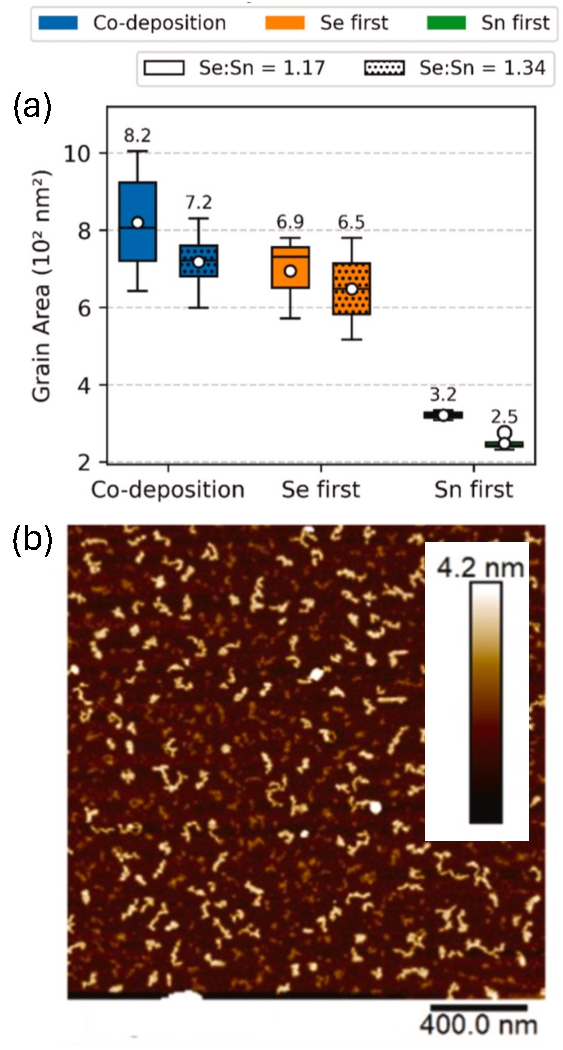
\includegraphics[width=\linewidth]{images/afm-stats.pdf}
    \caption{Sample data from 2DCC. (a) Statistical measure of grain area. (b) Representative AFM height map. Adapted from Ref.~\citenum{chin2025analyzing}.}
    \label{fig:afm-stats}
    \vspace{-3mm}
\end{wrapfigure}

\textbf{Industrial Dataset Selection and Preparation:}
Reinhart and Zuo will prepare subsets of their industrially relevant datasets for curricular use. 
Reinhart will contribute extant ML-ready datasets (currently hosted open-access on Penn State ScholarSphere) from the 2DCC-MIP Lifetime Sample Tracking (LiST) database, which in total contains data on over 20,000 2D material samples~\cite{moses2024crystal, moses2024quantitative, moses2024transfer, moses2025cross}.
These are mostly Atomic Force Microscopy (AFM) height maps (e.g., \autoref{fig:afm-stats}) with associated metadata and naturally support high school statistical modeling topics such as empirical probability distributions, linear correlations, and hypothesis testing without requiring knowledge of condensed matter physics.
The data packages inherently feature statistical complexity (image noise, measurement variance), structural complexity (high-dimensional process variables), and provenance artifacts (systematic calibration drift, missing values due to characterization costs, and authentic data entry errors). 
Students working with these datasets will encounter the same data quality decisions that practicing scientists face.
Furthermore, they offer a highly visual pathway to introduce students to the concepts of nanotechnology and advanced electronics whose function arises from structure at the smallest length scales.

Zuo will contribute high-dimensional time-series datasets from NSF-funded cyber-physical research on building energy systems, including a campus-scale district cooling network~\cite{hinkelman2022fast} and a university data center cooling system~\cite{fu2019equation}.
Sensor records of temperatures, flow rates, pressures, and electricity consumption will provide accessible entry points for Algebra and Statistics curricula, enabling students to fit linear or piecewise models, analyze residuals, and quantify periodic patterns in energy loads.
These datasets offer rich examples of physically implausible readings from sensor drift (statistical complexity), dozens of correlated mechanical and weather variables (structural complexity), and communication dropouts or operator-embedded decisions (provenance artifacts)~\cite{anbarasu2025optimal}. 
Beyond mathematics, the datasets introduce students to the energy infrastructure underlying AI systems, grounding abstract modeling tasks in the physical systems that make modern computation possible.
The datasets thus represent facets of NSF research infrastructure with immediate industrial relevance.
By navigating them, students will gain a window into the future of America's AI infrastructure at the information-energy-materials nexus, inspiring future careers in the area.

\textbf{Python Notebook Framework:}

\begin{wrapfigure}{r}{0.45\linewidth}
    \vspace{-6mm}
    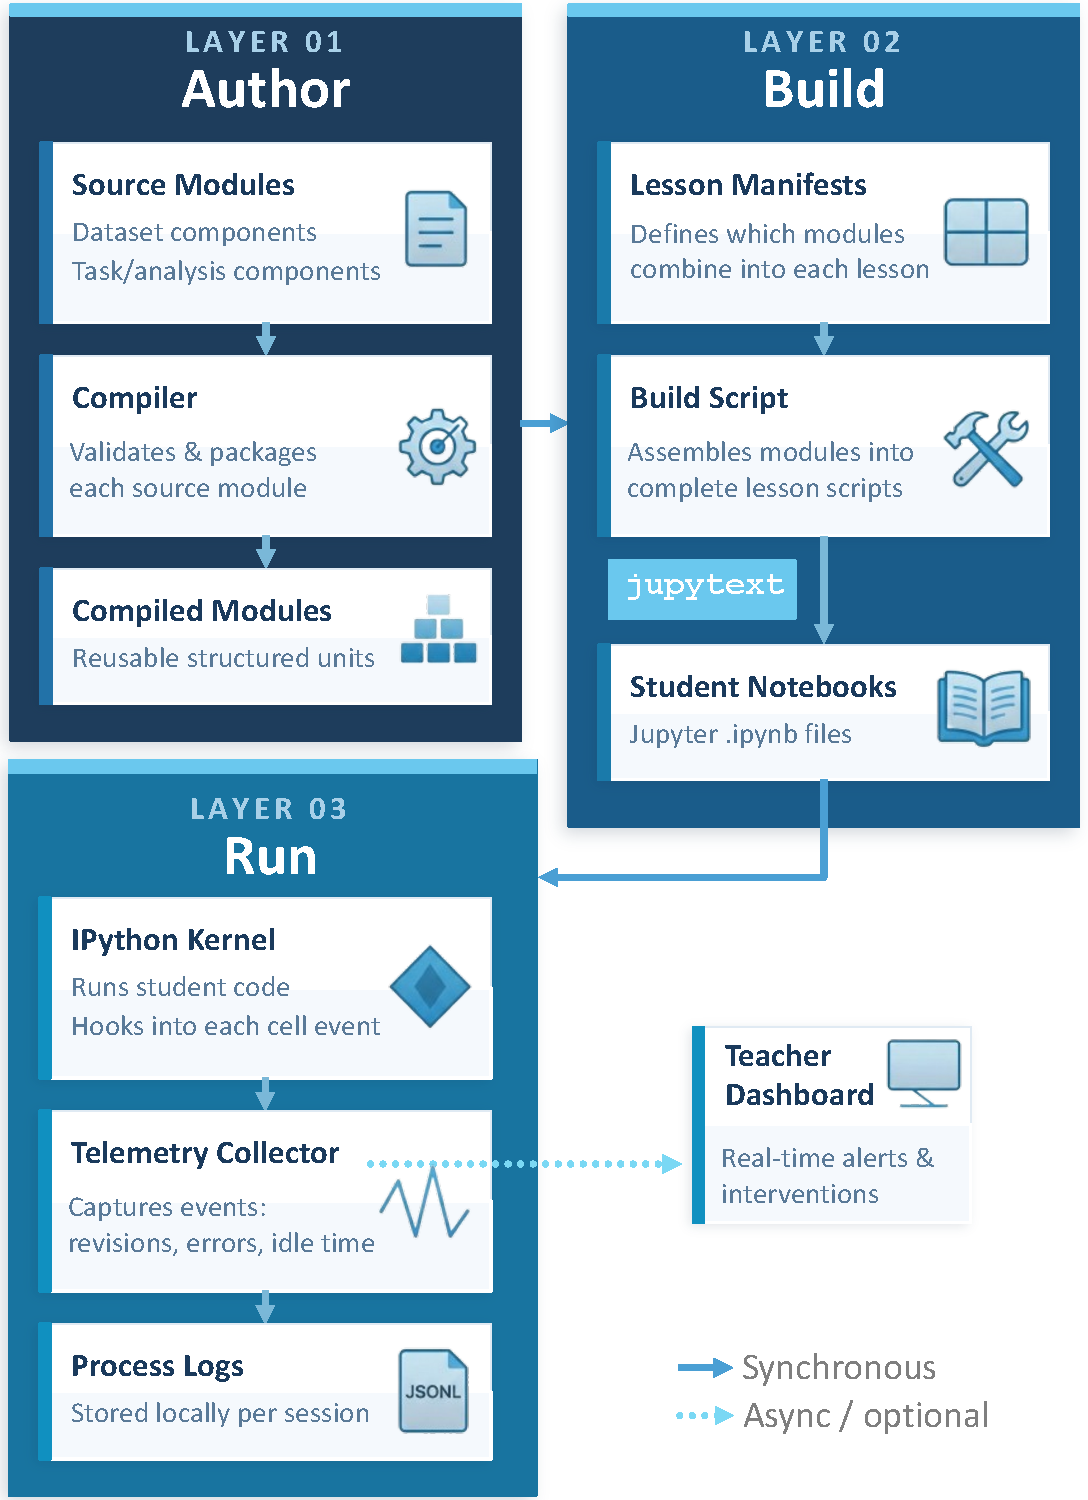
\includegraphics[width=\linewidth]{images/camel_pipeline.pdf}
    \caption{Reinhart's Composable Courseware architecture (L01-02 implemented and deployed, L03 prototyped for this proposal).}
    \label{fig:composable-courseware}
    \vspace{-4mm}
\end{wrapfigure}
The Python-based learning environment will have two layers: a Composable Courseware authorship layer developed by Reinhart (cf. \autoref{fig:composable-courseware}) will implement reconfigurable educational modules and a telemetry layer developed by Napolitano will capture high-resolution, process-level analytics by hooking directly into the IPython kernel.
The Composable Courseware layer will enable the modular construction of plug-and-play components from standardized entities like context, dataset, model, and analysis components.
The components will be built in python script files and assembled into Jupyter notebooks through a lightweight ``compiler'' via yaml manifests.
An agentic AI tool will assist in patching rough transitions and updating specific numbers within explanatory markdown cells.
This approach will enable reusable modules such as feature attribution techniques to be applied to a wide range of datasets and model architectures with minimal manual authorship and maintenance.
Modularity is an essential element of the proposed framework since the educational contexts will vary in their learning goal and target complexity.

Meanwhile, the telemetry framework will record timestamped revision histories and utilizes automated listeners to track debugging sequences, specifically flagging ``unproductive frustration'' when a student triggers consecutive errors in a single cell or remains inactive for multiple minutes.
These telemetry data (model iteration trajectories, student annotations, etc.) will be transmitted via asynchronous API calls to a centralized FastAPI backend.
This will allow for the real-time visualization of student progress on a teacher dashboard, enabling immediate pedagogical intervention when students deviate from productive modeling pathways.
Also note the telemetry is just kB/s network traffic and should not require high bandwidth.

\begin{table}[h]
\footnotesize
\centering
\caption{Data Source Alignment and Research Utility}
\label{tab:data_mapping}
\begin{tabular}{|p{3.5cm}|p{5cm}|p{6.5cm}|}
\hline
\rowcolor{mycmykcolor} 
\textbf{Data Source} & \textbf{Primary Metrics} & \textbf{Research Utility} \\ \hline

Python Notebook Process Data & Error frequency, idle timers, timestamped cell diffs & Identifies idle states and maps iterative trajectories of model development. \\ \hline

Pre/Post Assessments & Modeling competency scores, statistical reasoning gains & Quantifies longitudinal growth in mathematical modeling and data literacy. \\ \hline

Student Work Artifacts & Qualitative reflections, variable justifications & Reveals internal reasoning patterns and latent cognitive moves behind the code. \\ \hline

Classroom Observation Data & Teacher intervention frequency, peer discourse patterns & Correlates technical struggle with social support and real-world classroom dynamics. \\ \hline

\end{tabular}
\end{table}

\textbf{Teacher Professional Development:} 
The proposed PD model integrates content-intensive summer institutes with monthly virtual Networked Evaluation and Improvement Community (NEIC) structured academic-year follow-up, building rural Pennsylvania high school mathematics teachers' capacity to use authentic data in instruction.
The CSATS education team (Hill, Cesare, a computer science/AI education specialist, and Mayne) collaborates with STEM research faculty and the mathematics education research team to design institute curriculum incorporating the five features of effective PD: content focus, active learning, coherence with teachers' existing knowledge and school context, sustained duration, and collective participation \cite{DarlingHammond2017}.

During one-week summer institutes at Penn State, teachers work directly with materials science and architectural engineering faculty and their research data, engaging in the end-to-end modeling cycle \cite{Garfunkel2019}: identifying variables, making assumptions, formulating models, testing predictions against authentic data, and revising models in light of discrepancies. Through this process, teachers experience firsthand what makes these datasets feel messy, building the content knowledge and pedagogical confidence needed to facilitate similar experiences with their students. The CSATS team and Mayne then facilitate the translation of these experiences into classroom-ready tasks, drawing on their expertise in curriculum development and, in Mayne's case, direct experience teaching high school mathematics. Because Pennsylvania school districts retain local control of curricular decisions, participating teachers integrate the modeling modules into existing math courses (e.g., Algebra, Statistics) in ways that maximize authenticity of the learning experience. 

During the academic year, teachers participate in a NEIC organized and facilitated by CSATS. 
% The NIC structure is particularly valuable in the rural context, where geographic isolation limits access to professional learning communities and disciplinary expertise; by connecting teachers across districts, the network creates a community of practice that would not otherwise exist. 
Monthly virtual meetings provide structured opportunities to share implementation experiences, examine student work, and engage in Plan-Do-Study-Act (PDSA) cycles \cite{Bryk2015}. Hill, Cesare, the computer science/AI education specialist, and Mayne provide ongoing instructional support as teachers implement modeling activities.%, helping them troubleshoot challenges, adapt tasks to local contexts, and maintain fidelity to the mathematical modeling framework. 
The NEIC serves as a built-in ``Practitioner Review Board." Quarterly implementation audits will be conducted, during which teachers provide structured feedback on the usability of the Data Translation framework, which will inform technical development for the subsequent semester.
The PD sequence will span two academic years.
Year 1 will include the initial summer institute with 10 math teachers and the first cycle of NEIC activities.
Year 2 will add the remaining 35 math teachers, with refined tasks based on Year 1 classroom evidence and mentoring of incoming cohort members by Year 1 participants. 
This sustained, iterative structure will ensure teachers develop the deep pedagogical content knowledge required to facilitate authentic mathematical modeling. 
To mitigate teacher variability across districts, the project utilizes a standardized fidelity of implementation (FoI) protocol. 
This framework prevents over-scaffolding, where a teacher might curate data for classroom convenience.
% Implementation consistency is monitored through monthly NIC meetings where teachers use shared Plan-Do-Study-Act (PDSA) cycles to align their instructional moves with the project’s modeling framework.
Each dataset entry is also tagged with a teacher-reported fidelity rating and cross-referenced against telemetry to account for pedagogical variations during analysis.

\textbf{Teachers as Co-Researchers:}
This project positions teachers as co-researchers within a research-practice partnership (RPP) model \cite{Coburn2013, conrad2015educating}.
Rather than serving solely as implementers of course materials, teachers are integral members of the research team who contribute expertise, collect and annotate data, and participate in the analysis and interpretation of findings \cite{Penuel2017}.
Working with Hill and Mayne, we will train teachers in research protocols, data ethics, and systematic documentation, developing their capacity to ensure that engineering data remains authentic, that data collection protocols are implemented with the fidelity required for valid research conclusions, and that student work is properly documented and annotated according to project standards.
This practitioner-as-researcher model transforms the traditional relationship between researchers and teachers \cite{CochranSmith2009}, creating a partnership in which practitioners contribute substantive intellectual value to the research enterprise. 

% During the summer institutes, teachers are trained in structured observation and documentation protocols developed collaboratively by the research team and education practitioners. 
% These protocols guide teachers in capturing student reasoning as it unfolds during mathematical modeling tasks, including how students formulate assumptions about engineering data, how they respond to unexpected variability, where they encounter conceptual difficulties, and what strategies they employ to reconcile model predictions with observed data. 
Specifically, teachers will learn to annotate student work samples and classroom artifacts using a shared coding framework, producing richly contextualized records that form the core of the project's novel data set.
% Participating teachers also make instructional decisions about how to integrate the modeling modules into their existing mathematics courses (e.g., Algebra, Statistics), ensuring that the learning experience reflects the constraints and opportunities of each classroom context. 
% During the academic year, teachers collect data systematically in their own classrooms as they implement modeling tasks with authentic engineering data sets. 
% This data collection is embedded within the PDSA cycles of the NIC \cite{Bryk2015}: as teachers test instructional approaches, they simultaneously generate annotated records of student reasoning that serve both the improvement goals of the network and the research goals of the project.
% Teachers bring student work, observational notes, and reflective analyses to monthly NIC meetings, where they collaboratively examine patterns in student reasoning across school contexts. 
This dual role, practitioner and researcher, will ensure that the resulting data set captures the complexity of real classroom implementation, including the contextual factors that shape student engagement in rural schools such as prior preparation, course sequencing, technology access, and the relationship between tested content and modeling instruction. 
Teachers will also participate in data analysis during the Year 2 summer institute, working alongside Penn State researchers to identify emergent themes in student reasoning trajectories, propose refinements to the coding framework, and co-author findings for dissemination.
This co-researcher model strengthens the ecological validity of the data set by grounding data collection in the professional judgment of experienced classroom teachers \cite{Henrick2017} and builds research capacity among rural educators who often have limited access to research partnerships.
% The resulting data set will reflect the perspectives of both researchers and practitioners, enhancing its value for the CAMEL Collaboratory and future AI applications in mathematics education research. 

\vspace{-0.2cm}
\begin{tcolorbox}[colback=mycmykcolor, colframe=black, boxrule=1pt, coltext=black]
\vspace{-0.2cm}
\textbf{Task 2: Dataset Generation and Curation}
(Years 1–3) will generate the AI-ready Student Math Modeling Learning Dataset, containing tens of millions of events.
\vspace{-0.2cm}
\end{tcolorbox}
\vspace{-0.1cm}

\textbf{Primary Data Collection:}
The core dataset captures a multi-dimensional view of student engagement with mathematical modeling across diverse high school contexts, utilizing a mix of automated telemetry and traditional pedagogical artifacts. 
Central to this is the Python Notebook Process Data, which utilizes an embedded telemetry framework (\autoref{fig:telemetry}) to capture timestamped revision histories, debugging sequences, and iterative code execution patterns.
This system will identify specific behavioral markers, such as productive struggle through error-loop monitoring and inactivity timers, which are streamed via a FastAPI backend for real-time analysis.
To ensure data integrity, all sources are linked via Unique Session IDs and synchronized to a central server clock.
This allows Classroom Observation Data, such as discourse patterns and teacher-student interactions, to be precisely overlaid with Student Work Artifacts and Pre/Post Assessments. 
By time-syncing qualitative observations with quantitative telemetry, the framework provides the necessary context to ground automated analytics in real-world classroom dynamics.

\begin{wrapfigure}{r}{0.5\linewidth}
    \vspace{-3mm}
    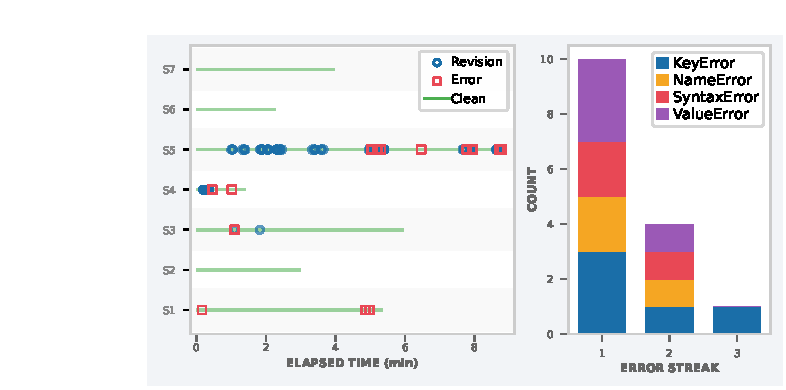
\includegraphics[width=\linewidth]{images/telemetry_infographic_crop.pdf}
    \caption{Telemetry from the proposed system, proof-of-concept demo statistics.}
    \label{fig:telemetry}
    \vspace{-4mm}
\end{wrapfigure}

\textbf{Sample Size and Justification:}
We target 4,500 students across the project period.
Process-level data from authentic modeling tasks generates substantially more training instances than traditional outcome data.
With students engaging in dozens of notebook sessions over a semester, and each session producing potentially hundreds of timestamped execution events, \textbf{the project can realistically yield tens of millions of annotated events}.
This multi-session, longitudinal volume (several 10's of GB of raw JSONL telemetry) provides sufficient scale for machine learning analyses and proof-of-concept predictive modeling.
Regarding statistical power for RQ1-RQ2, for detecting medium effect sizes (Cohen's d = 0.5) in pre/post gains with power = 0.80 and $\alpha$ = 0.05, we require approximately 64 students per comparison group.
Our sample of 4,500 provides adequate power for subgroup analyses (e.g., by prior preparation level, school type) with several dozen subgroups.

\textbf{Recruitment Strategy:}
To ensure the dataset is representative of all K-12 learners, we implement a phased strategy targeting geographic and socioeconomic diversity.
In Year 1, we pilot data collection in one Title I school and one rural school, with approximately 100 students total, allowing us to refine protocols before scaling to all listed sites in Years 2-3.
Recruitment prioritizes schools with high percentages of Free or Reduced Price Lunch and those located in federally designated rural locales, ensuring the dataset accurately captures the reality of mathematical modeling in the full breadth of American educational contexts.

\textbf{Dataset Evaluation:}
Annotation reliability will be established through double-coding of 20\% targeting Cohen's $\kappa \geq 0.70$  with iterative codebook refinement by Yao and Napolitano's teams ensuring categories are theoretically grounded and interpretable by educators. For robustness, we will conduct cross-site validation to confirm that reasoning pattern distributions and annotation reliability hold consistently across schools, teachers, and demographic subgroups, flagging site-specific anomalies for documentation. For viability, the Year 3 proof-of-concept classifier will serve as a validation of the dataset's utility for machine learning applications, demonstrating that process-level features are sufficiently structured to train and evaluate predictive models. For bias, we will audit whether annotation codes are applied consistently and whether modeling tasks systematically advantage students with particular prior experiences; any identified disparities will be documented in the dataset metadata and addressed through targeted codebook refinement before publication.

\vspace{-0.2cm}
\begin{tcolorbox}[colback=mycmykcolor, colframe=black, boxrule=1pt, coltext=black]
\vspace{-0.2cm}
\textbf{Task 3: Data Translation Framework and Annotation Protocols}
(Years 2–3) will develop the replicable ``Data Translation'' framework that enables complex engineering research data to be converted into K-12 pedagogical materials.
\vspace{-0.2cm}
\end{tcolorbox}
\vspace{-0.1cm}

 This framework is both a methodological contribution (RQ2) and a practical infrastructure for future CAMEL networks.
The Data Translation Framework is a documented protocol—not software—consisting of: (1) decision rubrics for dataset selection, (2) scaffolding templates, (3) learning analytics integration specifications, and (4) validation checklists. It will be published as an open-access methodological guide.
The Data Translation Framework rests on three foundational design principles that balance authenticity with accessibility. 
First, authenticity preservation requires that complexity along all three dimensions, statistical, structural, and provenance, be retained at levels that demand genuine reasoning, not cleaned into triviality. The framework specifies which complexities to preserve (such as realistic measurement error distributions) versus which to simplify (such as reducing 50 variables to 8 while maintaining correlational structure), ensuring students encounter the essential challenges of real-world data without becoming overwhelmed by irrelevant complications. 
Second, mathematical alignment ensures each translated dataset maps to specific Common Core mathematical practices and content standards, with practitioners validating that the mathematical demands match course-level expectations. 
This grounding in standards enables seamless integration into existing curricula while maintaining pedagogical coherence. 
Third, scaffolded complexity provides entry points for students at different preparation levels through framework-specified ``complexity dials'' that teachers can adjust, allowing the same core dataset to serve diverse classroom contexts without sacrificing the authentic reasoning opportunities that make industrial data pedagogically valuable.

These complexity dials operate primarily as interface filters rather than transformations of the underlying data. 
The core idea is that each dimension can be tuned: structural complexity is the number of variables visible to students; provenance complexity is whether data quality issues (missing values, flagged anomalies) are surfaced for student reasoning or pre-resolved; and statistical complexity is whether noise characteristics are made explicit. 
For instance, the composable courseware layer enables adjustments to the number of variables being considered or methodological complexity in a plug-and-play manner, simply swapping one module (e.g., MoS2 data $\cdot$ univariate $\cdot$ linear regressor) for another (e.g., MoS2 data $\cdot$ univariate $\cdot$ Gaussian Process regressor or MoS2 data $\cdot$ multivariate $\cdot$ linear regressor).
This module-swapping feature is a structural complexity dial in action: the dataset and model class are constant, but the operational scope widens.

The real-time learning analytics system functions as a lightweight feedback mechanism embedded directly within the Python notebook environment, providing tailored insights for students, teachers, and researchers.
For students, the platform offers visual indicators such as residual plots and $R^2$ displays that update as they modify their code, allowing them to monitor how well their current model fits the data in real time. 
Teachers will benefit from a centralized dashboard that tracks class-level progress and identifies students who may need intervention, such as those who have not made code changes for extended periods or have deleted substantial portions of their work.
Finally, for researchers, the system will capture all logged events with precise timestamps, feeding this information into a comprehensive process-level dataset for further analysis.

To ensure the dataset catalyzes the development of intelligent tutoring systems and formative assessment tools, Yao and Napolitano will develop annotation protocols strictly aligned with existing learning analytics standards, such as xAPI and Caliper where applicable. 
These protocols will utilize Reasoning Pattern Codes grounded in mathematical modeling literature to categorize cognitive moves like assumption-making, variable identification, and validation.
To further refine the diagnostic capabilities of the system, a comprehensive Error Taxonomy will be built upon statistics education research to classify specific data handling, modeling, and interpretation errors. 
Furthermore, the framework will include indicators, such as specific revision cycles and exploratory code patterns, to distinguish beneficial academic challenges from unproductive frustration. 
Finally, these protocols will be supported by automated Model Quality Metrics that extract fit statistics and code quality indicators, providing a multi-dimensional view of student performance.

Annotation categories will further be organized along the three complexity dimensions. 
For statistical complexity, the Error Taxonomy captures misconceptions about variance, outlier treatment, and inferential claims. 
For structural complexity, Reasoning Pattern Codes capture variable selection logic, dimensionality reduction decisions, and feature justification. 
For provenance artifacts, a dedicated Provenance Reasoning category captures how students identify, interpret, and respond to data quality issues. Productive Struggle Indicators are similarly dimension-specific: confusion about noise distributions, difficulty navigating feature spaces, and uncertainty about data provenance can each produce distinct behavioral signatures in the telemetry.
In Year 3, we will train a simple classifier (e.g., random forest or logistic regression) to predict productive vs. unproductive struggle from process features, demonstrating the dataset's utility for AI applications. This is a proof-of-concept, not the primary contribution, but it will validate our AI-ready claims.

\vspace{-0.2cm}
\begin{tcolorbox}[colback=mycmykcolor, colframe=black, boxrule=1pt, coltext=black]
\vspace{-0.2cm}
\textbf{Task 4: Data Sharing and Phase II Preparation}
(Year 3) will ensure broad impact and prepares the network for Phase II participation.
\vspace{-0.2cm}
\end{tcolorbox}
\vspace{-0.1cm}

\textbf{Data Sharing and Promotion Plan:}
The complete dataset will be published on FAIR-aligned repositories, specifically ICPSR and the Open Science Framework, with comprehensive metadata, persistent DOIs, CC-BY licensing, and sample analysis scripts with tutorial notebooks so researchers can run meaningful analyses within hours of access. To actively promote adoption, we will host a public dataset release webinar, maintain a project website with documentation and a researcher forum, and submit dataset descriptor papers to venues such as the Journal of Educational Data Mining and NeurIPS education workshops, with sample training pipelines deposited on GitHub. For academic dissemination, primary empirical findings will target the Journal of the Learning Sciences and Cognition and Instruction, while methodological contributions on the Data Translation framework will be submitted to the Journal of Research in Mathematics Education and Educational Researcher, with conference presentations including the International Conference of the Learning Sciences (ICLS), the annual meeting of the National Association for Research in Science Teaching (NARST), and the Psychology of Mathematics Education (PME) ensuring visibility across disciplinary boundaries. For practitioner audiences, Hill and Mayne will develop practitioner-facing guides and workshops disseminated through CSATS networks and the Pennsylvania Council of Teachers of Mathematics, ensuring the Data Translation framework reaches classroom teachers directly. Reuse will be tracked through DOI citations and OSF download metrics.

\textbf{Phase II Collaboratory Engagement:}
Network representatives will engage in CAMEL cross-network activities throughout the project, participating in Ideas Lab and inter-network working groups to contribute to the design of the Phase II collaboratory infrastructure.
We will advocate for integration of our dataset into the Phase II collaboratory's shared infrastructure, ensuring it is discoverable and usable by all CAMEL networks as a common resource.
By Year 3, the network will prepare a Phase II proposal that leverages our established data infrastructure, school partnerships, and demonstrated capacity to generate high-quality learning datasets at scale.

%%%%%%%%%%%%%%%%%%%%%%%%%%%%%%%%%%%%%%%%%%%%%%%%%%%%%%%%%%%%%%%%%%%%%%%%%%%%%%%
% SECTION: DATASET DESCRIPTION
%%%%%%%%%%%%%%%%%%%%%%%%%%%%%%%%%%%%%%%%%%%%%%%%%%%%%%%%%%%%%%%%%%%%%%%%%%%%%%%

\section{Dataset Description and High-Value Rationale:}
\label{sec:dataset}

The project will generate a multi-layered, AI-ready Student Math Modeling Learning Dataset designed to fill an important gap in mathematics education research. 
The dataset will comprise five interconnected layers designed to support both learning sciences research and machine learning applications.
The foundation is process-level analytics: timestamped Python notebook revision histories, debugging sequences, and code execution patterns that reveal the iterative logic of problem-solving as students work with real-world mathematical modeling challenges.
Because the dataset will include dozens of sessions per student over a semester, these timestamped histories map not only intra-task debugging cycles, but also long-term longitudinal growth in computational thinking.
These process data will be complemented by pre- and post-assessments using validated instruments that measure statistical reasoning, algebraic modeling competencies, and data literacy, enabling researchers to connect process trajectories to learning outcomes. 
Student artifacts (written reflections, model documentation, final project submissions, etc.) will provide qualitative depth that illuminates the reasoning behind observed coding behaviors.
Instructional metadata will capture the contextual factors essential for interpretation: student demographics, task sequences, teacher characteristics, and implementation fidelity ratings.
Finally, structured annotations will layer expert-coded reasoning patterns, error types, and misconception labels onto the process data, formatted specifically for machine learning model training.

Unlike existing product-data resources, this dataset will capture process data; it represents a high-value contribution to the field for four interconnected reasons.
First, it will close a documented gap that existing datasets cannot fill: unlike existing resources that document interactions with structured problem, this dataset will capture student engagement with authentic industrial complexity whose real-world provenance and relevance make them messy in the student's experience, yet all the more likely to be encountered in real STEM careers. 
Second, the dataset will capture process rather than just product: revision histories reveal the ``hidden logic'' of mathematical modeling development—the deleted attempts, debugging cycles, and iterative refinements that are invisible in traditional outcome measures but essential for understanding how competencies develop.
Third, the dataset will be AI-ready by design: structured annotations for reasoning patterns and error types will follow established learning analytics standards and are specifically formatted to enable training of next-generation intelligent tutoring systems and formative assessment tools optimized for authentic data contexts.
Fourth, the sampling strategy will enable genuinely representative research: by recruiting across rural and small suburban contexts, with demographic and socioeconomic diversity across participating districts, we will ensure findings generalize broadly -- unlike existing data concentrated in populations of specific tutoring systems.

The released dataset will comprise five linked components: (1) process-level notebook telemetry, (2) pre/post assessments, (3) student work artifacts, (4) classroom and implementation metadata, and (5) structured expert annotations. 
Data will be distributed in open formats, including JSON/JSONL for event telemetry, CSV for tabular assessment and metadata files, and documented notebook/script formats for curricular materials and sample analyses.
These details are included in the Data Management and Sharing Plan.
At full scale, it will describe approximately 4,500 individuals and tens of millions of event records.
Data quality will be supported through annotation reliability checks, cross-site validation, comprehensive codebooks, and schema documentation.

The dataset will fully comply with FAIR data principles. 
For findability, the dataset will be hosted on ICPSR and the Open Science Framework with persistent DOIs and machine-readable metadata that enable discovery through standard search mechanisms. 
For accessibility, the primary dataset will be open-access under CC-BY licensing, with tiered access protocols for sensitive demographic subsets that require data-use agreements.
For interoperability, data will be formatted in standard schemas—JSON for process data, CSV for assessments—compatible with Python, R, and common analysis tools, and aligned with existing learning analytics standards including xAPI and Caliper where applicable.
For reusability, the dataset will include comprehensive codebooks, sample analysis scripts, and tutorial notebooks demonstrating common research use cases, enabling researchers to begin productive work immediately upon access.

\textbf{Relationship to Existing Resources, Standards, and Integration:}
This dataset complements existing resources such as ASSISTments, PSLC DataShop, TIMSS, and NAEP by contributing process-level learning data from open-ended, authentic modeling tasks rather than product data from structured problem environments or large-scale assessments.
To support interoperability, telemetry and annotation metadata will align with xAPI and Caliper conventions where applicable, and all released files will use open, machine-readable formats with persistent identifiers and documented schemas.
The project will coordinate with CAMEL cross-network activities and the Phase II National Coordinator so that metadata, annotation rubrics, and documentation can be integrated into shared collaboratory infrastructure.

\subsection{PII Protection and Data Security}

Protecting student privacy while preserving analytical richness is a core design challenge given the sensitive nature of timestamped code, written reflections, and classroom observations.
The project will operate under Penn State IRB approval with informed consent from students and parents or guardians, with consent forms clearly specifying data uses, retention periods, and sharing protocols.

Our de-identification protocol will address unique challenges of process-level learning data.
We will partition the telemetry data into structural traces (timestamps, flags, error codes) and semantic traces (markdown, strings, written text).
Structural traces contain zero PII by construction and represent the vast majority of the telemetry data.
For semantic traces, direct identifiers such as names, school names, and specific dates will be removed or replaced with study IDs.
Automated scrubbing using pattern-matching algorithms will catch edge cases, with random sampling for manual verification and algorithm tuning.
Written reflections will be reviewed and redacted for identifying information before annotation, and classroom observation data will use participant codes throughout with no video or audio recordings included in the final shared dataset.

Recognizing that different research applications require different levels of demographic specificity, we will implement a tiered sharing model.
The public tier will provide fully de-identified process data with aggregate demographic categories, sufficient for most machine learning training applications and the majority of research questions.
The restricted tier will provide fine-grained demographic data through formal data use agreements, enabling research requiring intersectional analysis while maintaining appropriate protections.
All data collection will use encrypted transfer protocols, with raw data stored on Penn State's secure research infrastructure and access limited to IRB-approved personnel. 
De-identification will occur before any data leaves secure storage, ensuring that potentially identifying information never exists in accessible repositories.

\subsection{Ethical Framework for Real-Time Telemetry and Intervention}

While the telemetry system provides real-time ``unproductive frustration'' alerts to the teacher dashboard, a strict ethical protocol will distinguish pedagogical support from invasive surveillance.
This framework is governed by three primary constraints designed to protect student agency and privacy.
First, the system will utilize Non-Evaluative Monitoring; telemetry data, including error streaks and inactivity timers, is used exclusively for formative ``just-in-time'' support and is never utilized for formal grading or evaluation.
Second, the project will maintain a Teacher-in-the-Loop Agency model where the dashboard functions as a decision-support tool rather than an automated supervisor.
Teachers receive indicators and apply their professional judgment to determine if a student requires a technical hint, a conceptual pivot, or continued space for productive struggle.
Finally, the project will ensure Data Transparency and Tiering; students are informed during the consent process that their coding trajectories are being mapped to improve the software's responsiveness.
In the classroom, the teacher dashboard will display aggregate class-level progress by default, with individual ``stuck'' states accessible only to facilitate immediate, private intervention.

\customsection{Broader Impacts:}

\textbf{Workforce Development:}
The ultimate workforce impact of this project will be recursive rather than a traditional linear pipeline.
Students who develop data reasoning skills in these industrial contexts will grow into the technical workforce that builds and maintains the infrastructure and material substrates enabling AI-driven learning.
The AI-ready datasets generated by this project will catalyze the development of intelligent tutoring systems that improve the next generation of STEM education.
The project will intervene at the moment when students first encounter authentic data complexity, before expectations about data solidify into habits of professional practice.
% More generally, by immersing high school students in authentic AI-industry-adjacent contexts, this project will directly prepare learners for data-intensive STEM careers. 
Students will also gain hands-on experience with Python programming and data analysis, developing skills that transfer directly to data-intensive STEM careers.
Exposure to industry-adjacent data will connect abstract algebraic and statistical concepts to concrete career pathways in manufacturing automation, building systems engineering, and related fields.
The Data Translation framework will demonstrate to students how research data becomes practical knowledge, demystifying scientific practice and helping students see themselves as potential contributors to, not just consumers of, technical knowledge.

\textbf{Broadening Participation:}
We will employ a specific theory of change grounded in research on STEM identity: students who do not see themselves in traditional mathematics pathways often respond more positively to tangible applications and authentic problems than to abstract skill-building.
Our approach will implement this theory through intentional recruitment, curriculum design, and role modeling.
We will establish partnerships with Title I schools and schools serving populations historically underrepresented in STEM, targeting at least 50\% of participating schools to serve, e.g., rural, or first-generation college-going student populations.
The curriculum will emphasize industrial data contexts connecting to sectors with diverse workforces (building systems, manufacturing, infrastructure) rather than stereotypical technology-first framings that may feel exclusionary. 
Throughout implementation, practitioner team members Hill and Mayne will be visible to students as role models, supplemented by guest speakers from varied backgrounds working in data science careers.
To verify broad impact, we will administer pre- and post- surveys measuring STEM identity and career interest, with results disaggregated by demographic group to identify and address any differential effects.

\textbf{Research Infrastructure and National Priorities:}
The FAIR-compliant dataset (\autoref{sec:dataset}) will become a permanent shared resource, enabling secondary and meta-analyses in CAMEL Phase II.
% By hosting the open-access dataset on established repositories, we will enable secondary analyses that extend, replicate, and build upon our initial findings.
% The standardized annotation protocols developed through this project can be adopted by other CAMEL networks, creating the foundation for cross-dataset comparisons and meta-analyses in Phase II.
% Tutorial notebooks and sample analysis scripts will lower the barrier for researchers new to process-level learning data, expanding the community of scholars who can contribute to this emerging area.
This work will address CAMEL's specific program goals while also connecting to broader NSF and US Government priorities.
By generating AI-ready datasets specifically designed for educational applications, we will contribute to the national capacity for intelligent tutoring systems and formative assessment tools; and
by training practitioners and researchers in interdisciplinary methods, we build long-term K-12 STEM capacity that extends well beyond the project period.

%%%%%%%%%%%%%%%%%%%%%%%%%%%%%%%%%%%%%%%%%%%%%%%%%%%%%%%%%%%%%%%%%%%%%%%%%%%%%%%
% SECTION: PROJECT TIMELINE
%%%%%%%%%%%%%%%%%%%%%%%%%%%%%%%%%%%%%%%%%%%%%%%%%%%%%%%%%%%%%%%%%%%%%%%%%%%%%%%

\section{Project Timeline and Evaluation Plans:}

The project will span three years (January 2027 – December 2029).
Project management will be organized through task-aligned leadership for outreach and teacher development, data generation, technical infrastructure, and sustainability/dissemination, with regular coordination among these groups over the award period.
Evaluation will track operational progress (teacher recruitment and retention, implementation fidelity, milestone completion), dataset quality (annotation reliability, cross-site robustness, bias audits), and educational outcomes (pre/post gains in modeling competencies and related survey measures).
Additional procedural and evaluation details are provided in the Collaboration and Management Plan and CSATS Facilities documentation.

\begin{table}[h]
\footnotesize
    \centering
    \caption{Project timeline and evaluation plans}
    \vspace{-0.25cm}
    \begin{tabular}{|p{0.6cm}|p{4.5cm}|p{4.5cm}|p{5cm}|}
    \hline
    \rowcolor{mycmykcolor}
         \textbf{Task} & \textbf{Year 1} & \textbf{Year 2} & \textbf{Year 3} \\
         \hline
         \textbf{1} & Infrastructure development; Teacher PD; Initial curriculum deployment; Pre-assessment baseline; FoI protocol deployment & Continued implementation; Iteration based on Y1 data; Teacher PD effectiveness assessment; Post-assessment cycle 1 & Refinement; Scaling; Final post-assessments; STEM identity survey analysis \\
         \hline
         \textbf{2} & Pilot data collection (2 sites); Inter-rater reliability established & Full data collection (expanded sites); Cross-site annotation reliability checks; Iterative codebook refinement & Final collection; Dataset curation; Cross-site validation and bias audit \\
         \hline
         \textbf{3} & — & Framework development; Initial annotation protocols & Framework validation; Complete annotations; Proof-of-concept classifier validation; Dataset robustness assessment \\
         \hline
         \textbf{4} & Project website launch; CAMEL cross-network engagement begins & Conference presentations (ICLS, NARST, PME); Practitioner workshops via CSATS; Dataset descriptor paper submission & Full dataset publication (ICPSR, OSF); Dataset release webinar; Practitioner-facing guides; GitHub pipeline release; Phase II proposal preparation \\
         \hline
    \end{tabular}
    \label{tab:timeline}
\end{table}
%%%%%%%%%%%%%%%%%%%%%%%%%%%%%%%%%%%%%%%%%%%%%%%%%%%%%%%%%%%%%%%%%%%%%%%%%%%%%%%
% BIBLIOGRAPHY
%%%%%%%%%%%%%%%%%%%%%%%%%%%%%%%%%%%%%%%%%%%%%%%%%%%%%%%%%%%%%%%%%%%%%%%%%%%%%%%

\newpage
\bibliography{biblio.bib, ref_zuo.bib} 

\end{document}
